

\section{Introduction}
\label{sec:intro}

Benefiting from vast pre-trained corpora and parameters, large language models (LLMs) \cite{touvron2023llama,liu2023summary,touvron2023llama2} have demonstrated remarkable capabilities in general knowledge and linguistic expertise, achieving impressive results in multiple downstream tasks in natural language processing (NLP) field. With their success in NLP, the multi-modal community has seen many efforts utilizing pre-trained LLMs with additional visual encoding modules to accomplish multi-modal understanding. Some of these efforts have achieved fantastic performance in embodied agent~\cite{zhao2023see,zhao2024hierarchical,zhao2024we}, image~\cite{liu2023visual,li2023blip} and video~\cite{zhang2023video,chai2024auroracap,song2023moviechat,song2024moviechat+} question answering tasks. VideoLLaMA~\cite{zhang2023video} exhibits the capability to comprehend videos by integrating visual information. Existing LLM-based video understanding systems~\cite{song2023moviechat,song2024moviechat+,maaz2023video,zhang2023video} transform video information into a natural language question-answering-tokens format by using pre-trained large language models, image encoders, and newly added temporal modeling modules. In terms of temporal modeling, these methods typically adopt the training paradigms of video pre-training and video finetuning, as shown in Fig.~\ref{fig:intro}. In most cases, the goal of video pre-training with Video Caption tasks is to train video-based LMM into a large-scale general knowledge model, providing universal video understanding knowledge. 
% And it has achieved success on downstream VQA tasks.
\begin{figure}[!t]
    \centering
    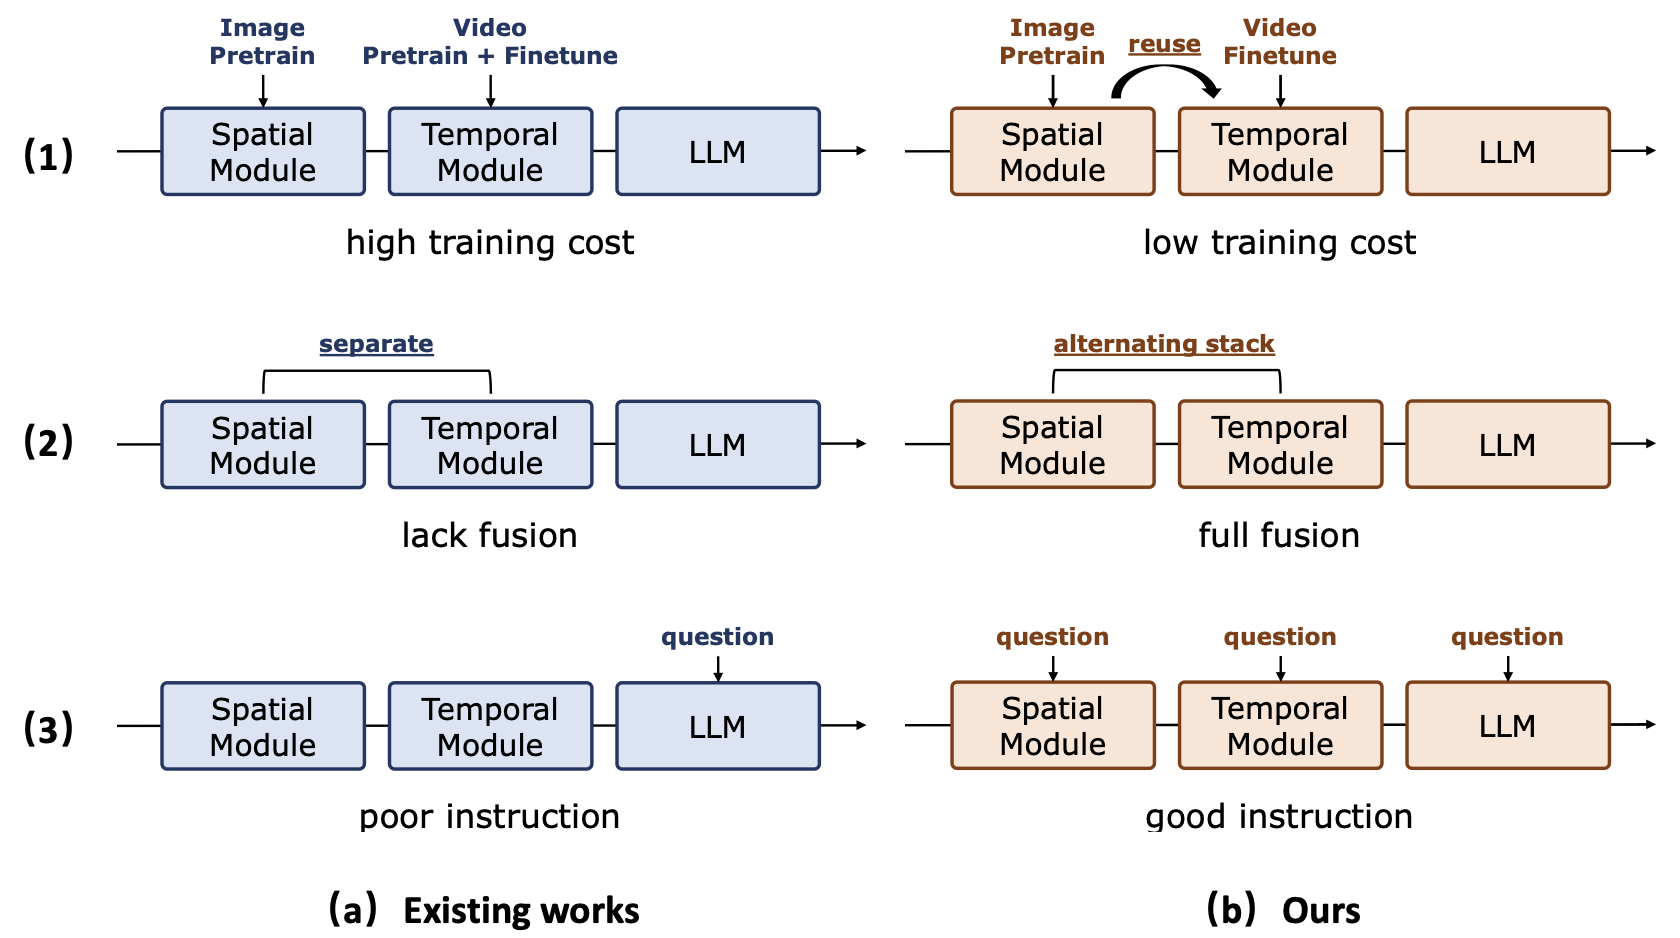
\includegraphics[width=0.5\textwidth]{figs/teaser.png}
    \caption{\textbf{Different temporal modelings for video LMMs}. \textbf{(1)} Common models adopt a three-stage approach involving image pre-training, video pre-training, and video finetuning. Training the temporal module during the video pre-training stage requires significant resources and may result in a gap with the finetuning task. Our approach eliminates the need for video pre-training by sharing parameters from spatial modules to temporal modules. \textbf{(2)} Common models separate spatial and temporal feature extraction modules in the video feature encoding, leading to high computational complexity and a lack of integration between temporal and spatial features at different levels. 
    % Research~\cite{bertasius2021space} indicates that 
    We adopt cyclic spatial-temporal feature interaction yields better performance. \textbf{(3)} Due to the absence of video-text pairs in many cases, common models do not perform multi-modal fusion during visual feature extraction. We employ the early multi-modal fusion in temporal modeling to achieve a detailed guide from text instruction.}
    \label{fig:intro}
\end{figure}


However, the video pre-training and finetuning scheme does not work well in some situations.
Training temporal modules during video pre-training tends to gradually erase the knowledge of visual features acquired from diverse image-text-based scenarios. This leads to reduced transfer performance when there is a large domain difference between downstream tasks and the video pre-training dataset.
When the downstream tasks, like the video sarcasm detection, significantly differ from the pre-trained video captioning tasks, 
the extracted general visual features during the video pre-training phase lack fine-grained information to guide the reasoning for downstream tasks, leading to poor performance.
% the lack of visual-text early fusion during the video pre-training phase means that the extracted general visual features lack fine-grained information, leading to poorer performance. 
In addition, the transfer performance decreases when the video scenes of the downstream tasks greatly differ from those in the pre-training phase. Due to the amount of video-text pre-training data volume being much smaller than the image-text pre-training data volume, the ability of video-based models to generalize across different video scenes degrades.
Furthermore, downstream task datasets are usually small-scale, making training video-based LMMs unaffordable. 
% For small-scale downstream task datasets, the cost of retraining a video-based LLM is unaffordable for most researchers. 

% To efficiently address these issues, we utilize an image-based LLM for efficient transfer to accomplish video understanding tasks.

To address the issues above, in this paper, we introduce MTransLLAMA, a new efficient temporal modeling framework that transfers pre-trained image-based LMMs~\cite{li2023blip} to video understanding tasks with only small-scale datasets, as shown in Fig.~\ref{fig:framework}. 
Our method enables fewer trainable parameters and achieves faster adaptation and higher accuracy than pre-training video-based LMMs.
% We opt to use a pre-trained image-based LLM to achieve better scene generalization and transfer its early multi-modal fusion capability to capture fine-grained visual information in videos based on text, thereby facilitating task transfer. 
We opt to use a pre-trained image-based LMM to achieve better scene generalization and adopt early multi-modal fusion to capture fine-grained visual information in videos based on guided text, thereby facilitating task transfer.
Specifically, we employ a pre-trained image-text Q-former for spatial modeling and introduce a low-rank adaptation (LoRA)~\cite{hu2021lora} in the attention layer. For temporal modeling, we directly transfer most of the Q-former’s attention layer parameters and perform attention operations across different dimensions, followed by fine-tuning with Lora. 
To better capture the global and local information of the data,
% To better transfer the interactivity of data, 
we also employ a dynamic routing-based transfer technique~\cite{zhou2021trar} to achieve dynamic shifting of sample attention.


Our main contributions can be summarized as follows:
\begin{itemize}
    \item We introduce a new temporal modeling framework of video-based LMMs, primarily focused on efficiently transferring to small-scale, fine-grained, domain-specific downstream datasets. By efficiently transferring a pre-trained image LMM into a video-based LMM model, our approach eliminates the need for a video pre-training phase and achieves better generalization.
    \item We propose a novel video multi-modal fusion structure that integrates spatial modeling, temporal modeling, and text-visual fusion within a single module, lifting the efficiency of spatial-temporal information fusion and multi-modal integration.
    \item We introduce a new transfer method that dynamically routes the attention weights in the Transformer across samples. Compared to traditional transfer techniques, this method is more effective in handling data with varying attention lengths.
    \item We demonstrate that our approach excels in training and inference costs, tunable parameters, computational complexity, and data requirements. It achieves state-of-the-art performance on various tasks such as Ego-centric QA and intent detection in multiple small-scale specific video scene datasets. 
\end{itemize}